\subsection{Readability}

% missing from graph paper
The Sugiyama Layout algorithm discussed in \cref{subsec:graphlayout} served the purpose of increasing visual clarity and readability of the TA outputted by TREAT.
Two of the most prevalent ways this was achieved was by layering the TAs states based on the length of the longest path from the initial state. The other was by ordering the states in each layer to achieve the smallest number of edge crossings.
While some of the specific approaches described by Mazetti et al. \cite{Mazetti2012} was not implemented into TREAT, the resulting implementation still greatly increases readability.

As mentioned in \cref{subsec:graphlayout}, the last step of the Sugiyama framework was not implemented, namely, properly positioning states in relation to each other. This might be developed in the future.

Another feature that would unequivocally improve readability is to visually separate transitions that share states, such as reversible transitions.
In all TAs pictured in \cref{subsec:graphlayout} and this section, any such transitions have been clearly separated, but this has not yet been implemented. The difference can be seen on \cref{fig:transitions}.

\begin{center}
    \usetikzlibrary {automata,positioning}
\scalebox{0.9}{
    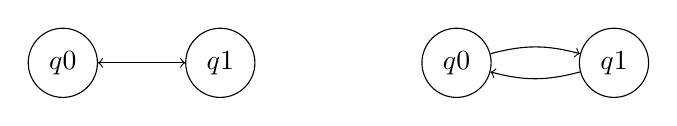
\begin{tikzpicture}[auto]
        \node[state] at (0, 0)(q0){$q0$};
        \node[state] at (2, 0)(q1){$q1$};
        \node[state] at (5, 0)(q2){$q0$};
        \node[state] at (7, 0)(q3){$q1$};

        \path[->]
        (q0)edge (q1)
        (q1)edge (q0)
        (q2)edge [bend left=15] (q3)
        (q3)edge [bend left=15] (q2)
        ;
    \end{tikzpicture}
}
\vspace{-1em}
\captionof{figure}{Comparison between implementation(Left) and intended behaviour(Right)}
\label{fig:transitions}
\end{center}

% formats
As described in \cref{output formats}, two output formats can be used to represent TAs.
The first format is UPPAAL. In UPPAAL, if no positions are given, the states are simply placed in a grid. This means, that using a graph layout algorithm is not strictly necessary.
To show its advantages, however, a comparison between UPPAAL's standard positioning and the one implemented in TREAT can be seen on \cref{fig:layout_comparison}, with UPPAAL on the top and TREAT on the bottom.
Do note, that the TAs in \cref{fig:layout_comparison} are only meant to show the positions of states, and are not representative of their appearance in UPPAAL.
% Should I just use screenshots from UPPAAL here? seems appropriate in this case

\begin{center}
    \input{Documents/Diagrams/ReadabilityFigures/uppaalLayout.tex}
    \input{Documents/Diagrams/ReadabilityFigures/treatLayout.tex}
\end{center}
\vspace{1em}

The other output format is TikZ, meant to represent graphs and the likes in LaTeX. Unlike UPPAAL, states in TikZ need positions, which necessitates some form of graph layout algorithm.


